\section{Input analysis}

\subsection{Inputs}
The stochastic inputs given to the model are divided into two categories: service times and routing descisions. Service times are all administrative and clinical processes done, while routing desicions capture the different paths patients go through the system. A third category, patient arrivals, are simplified to be deterministic, as they follow the patient schedule from Table 6 in the case \parencite{MillerPainTreatmentCenter}. All identified stochastic inputs are listed in \autoref{tab:stochastic_vars}.

\subsection{Extracting relevant data}

Service time data for the model is gathered from the spreadsheet given in the case \parencite{MillerPainTreatmentCenter}, which holds 90 - 100 observations of the variables used. Discrete distributions used for routing descisions such as no-show rate, patient type and follow-up consultation are taken from Dr. Weems observations in the case description. 

Both teaching variables and resident review (new) contain observations on 0-minute service times. As consultations always take time, these observations were removed before fitting. 

\subsection{Fitting appropriate statistical distributions}

\begin{figure}[H]
    \centering

    \begin{subfigure}{0.32\textwidth}
        \centering
        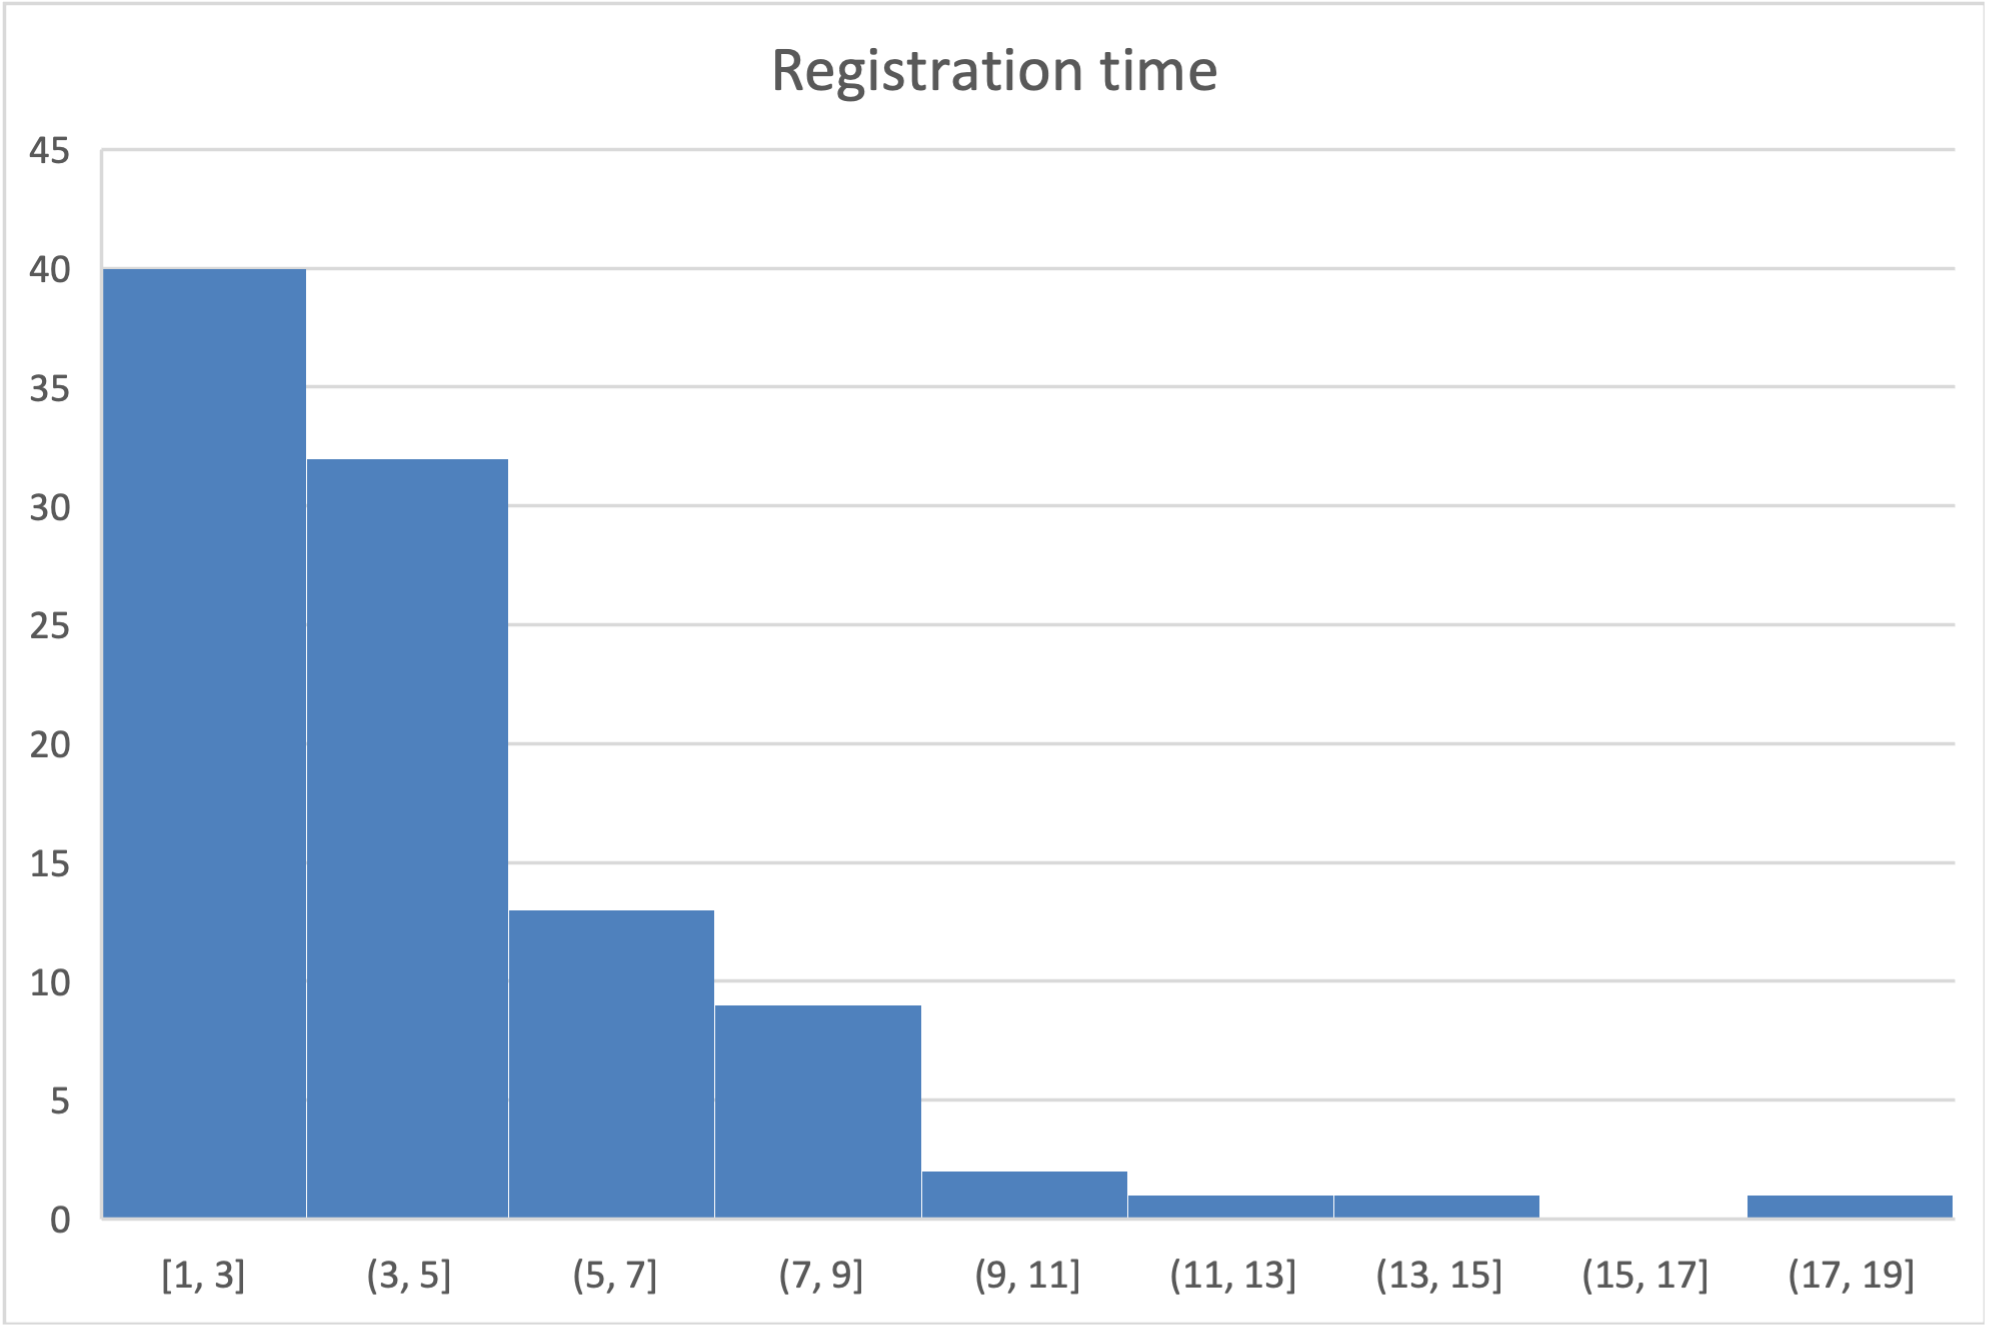
\includegraphics[width=\linewidth]{Inputs/Pictures/RegistrationTime.png}
        \caption{Registration Time}
        \label{fig:reg}
    \end{subfigure}
    \hfill
    \begin{subfigure}{0.32\textwidth}
        \centering
        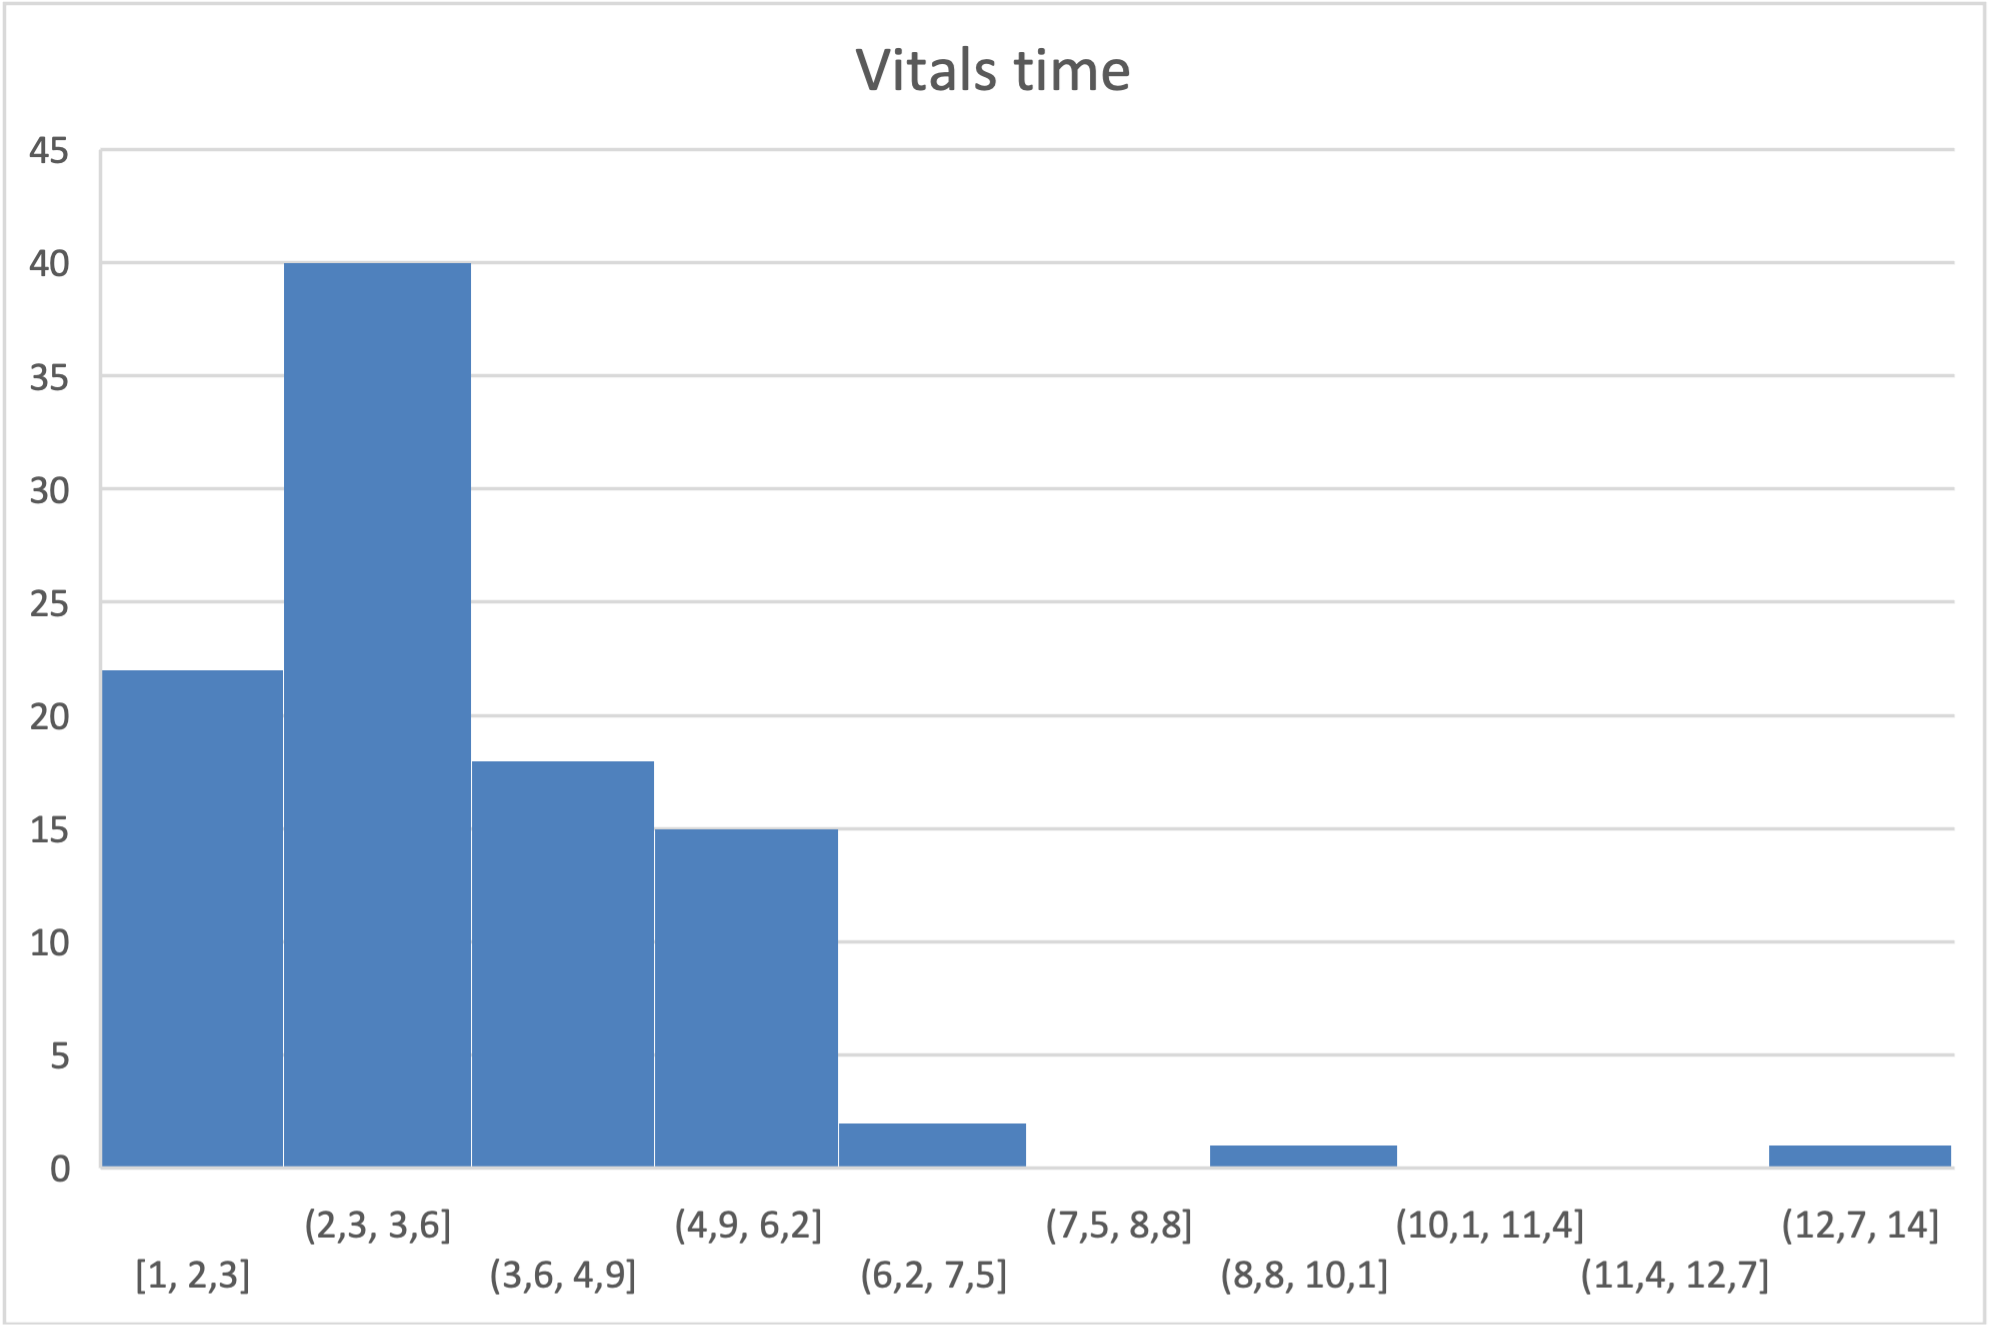
\includegraphics[width=\linewidth]{Inputs/Pictures/VitalsTime.png}
        \caption{Vitals}
        \label{fig:vitals}
    \end{subfigure}
    \hfill
    \begin{subfigure}{0.32\textwidth}
        \centering
        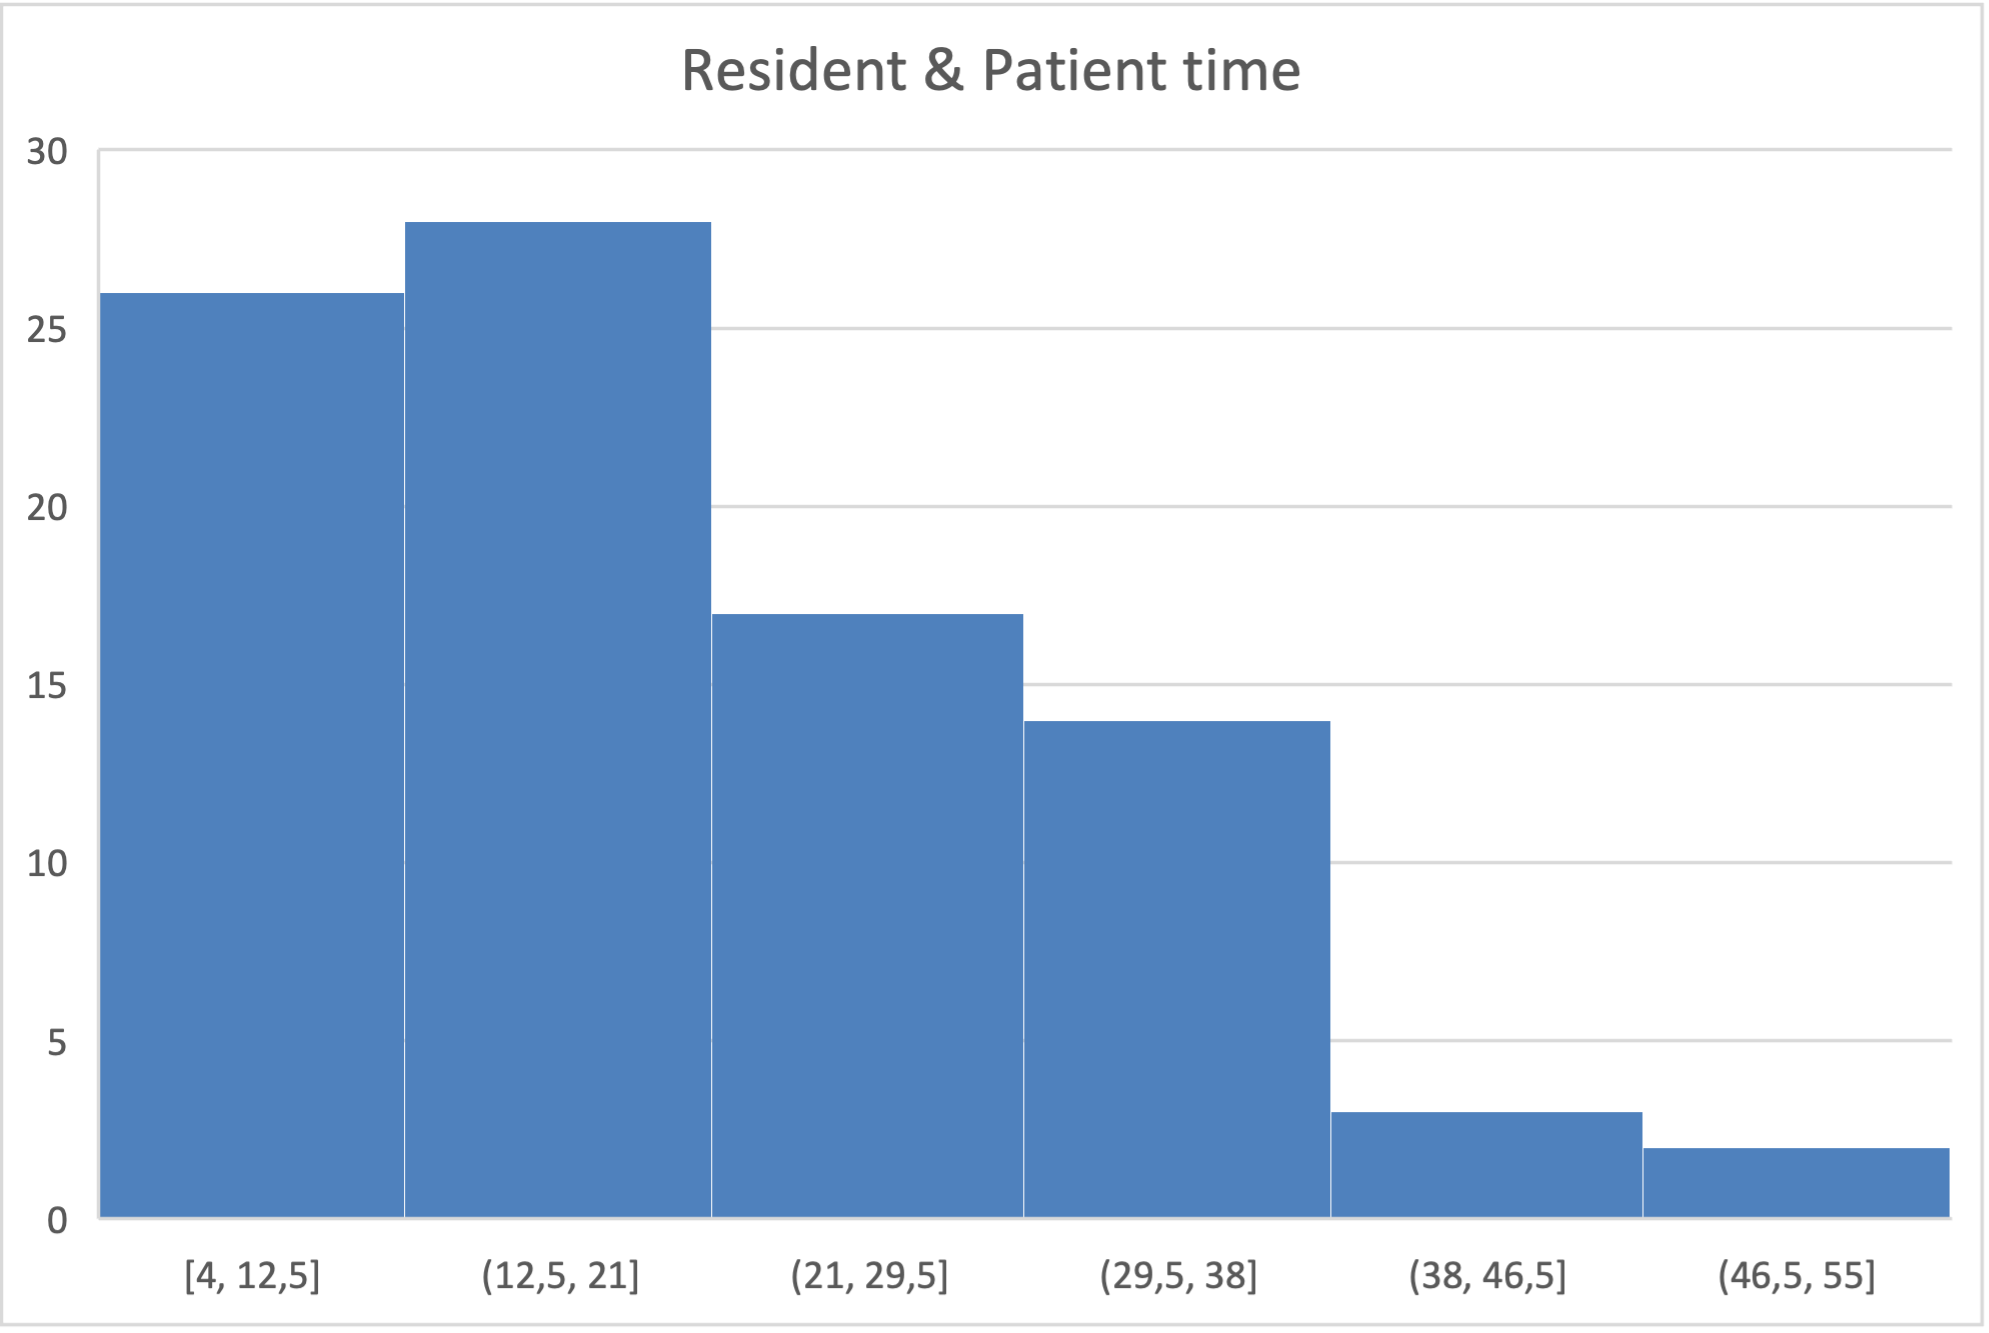
\includegraphics[width=\linewidth]{Inputs/Pictures/ResidentAndPatientTime.png}
        \caption{Resident \& Patient Time}
        \label{fig:resident}
    \end{subfigure}

    \caption{Service times}
    \label{fig:servicetimes}
\end{figure}

Visual inspection of the histograms can be used to identify the underlying shape of the data, which can the be compared to known theoretical distributions \parencite[p. 362]{pensumbok}. The histograms show a right-skewed form with a long long tail towards higher values. \autoref{fig:servicetimes} presents histograms for three representive variables. This suggests that distributions supporting right-skewed, positive data such as exponential, gamma, lognormal and weibull should be tested. 

All model parameters were fitted using maximum likelihood estimation (MLE), with a fixed location of 0. This is done to avoid negative distributions, as service times in minutes can not hold negative values.

\begin{figure}[H]
    \centering
    
\includegraphics[width=0.7\linewidth]{Distributions.png}
    \caption{Visual fit of distibutions}
    \label{fig:distribution}
\end{figure}

\autoref{fig:distribution} shows the histogram of registration times with fitted probability density functions. Gamma and lognormal provide the closest visual fit. Visuals and calculations are available in Calculations.ipynb, submitted with the report.

\subsection{Goodness-of-fit test}

The Kolmogorov-Smirnov test measures the largest absolute deviation between the empirical and theoretical cumulative probability distribution functions \parencite[p. 423]{pensumbok}. We evaluate each candidate distributions for every variable, selecting the one with the lowest KS-statistic among the ones passing the 5\% significance level. 

Gamma is selected for the variable registration, as it has the lowest KS-statistic with a sufficient significance level. As no candidate distribution passes for vitals, we pick the distribution yielding the lowest statistic, which is weibull. \autoref{tab:finalinputs} provides results for all variables.

\subsection{Discussing input assumptions}

Multiple assumptions are made regarding the input data. First, time is treated as continuously, although the spreadsheet presents them as integer minutes. Second, zero-valued observations are assumed to be a discrepancy rather than actual service times of zero minutes. Third, to avoid negative and zero-valued service times (as time in minutes can only be positive), all distributions are fitted with a location parameter of 0. Finally, service times are assumed to be independent for all patients and static throughout the simulation period.

\subsection{Final input model}

\autoref{tab:finalinputs} provides all variables with their distributions and parameters. 

\begin{table}[H]
\centering
\begin{tabular}{llcc}
\toprule
\textbf{Variable} & \textbf{Distribution} & \textbf{Shape} & \textbf{Scale} \\
\midrule
Registration & Gamma & 3.069 & 1.415 \\
Vitals & Weibull$^*$ & 2.107 & 3.982 \\
Physicians Assistant & Lognormal & 0.541 & 19.463 \\
Check Out & Gamma & 2.320 & 2.041 \\
Resident Review (New) & Gamma & 1.401 & 7.461 \\
Resident \& Patient (New) & Lognormal & 0.558 & 17.414 \\
Teach (New) & Gamma & 1.879 & 4.184 \\
Resident \& Attending (New) & Gamma & 2.831 & 4.401 \\
Resident Review (Return) & Lognormal & 1.002 & 5.678 \\
Resident \& Patient (Return) & Weibull & 1.740 & 14.665 \\
Teach (Return) & Weibull & 1.173 & 5.438 \\
Resident \& Attending (Return) & Lognormal & 0.738 & 6.974 \\
\bottomrule
\end{tabular}
\\[6pt]
{\footnotesize \textit{$^*$ No distribution with p $>$ 0.05, Weibull chosen as best fit}}
\caption{Final inputs with distributions and parameters}
\label{tab:finalinputs}
\end{table}